\section{Results}\label{sec:results}

\begin{table*}[t]
\caption{Illicit-class results on the test period (steps 35--49), mean $\pm$ std over seeds. Thresholds are tuned on the validation window. Best leakage-controlled value in bold.}
\label{tab:main}
\centering
\footnotesize
\begin{tabular}{@{}llccccccr@{}}
\toprule
Model & Features & F1 & Precision & Recall & PR-AUC & ROC-AUC & P@1\% & Fit (s) \\
\midrule
\multicolumn{9}{@{}l}{\textit{Leaky features (as in prior work)}} \\
RF & All & 0.799\,$\pm$\,0.007 & 0.902\,$\pm$\,0.020 & 0.717\,$\pm$\,0.003 & 0.788\,$\pm$\,0.001 & 0.927\,$\pm$\,0.002 & 1.000\,$\pm$\,0.000 & 28 \\
XGB & All & 0.803\,$\pm$\,0.004 & 0.902\,$\pm$\,0.012 & 0.724\,$\pm$\,0.002 & 0.796\,$\pm$\,0.002 & 0.928\,$\pm$\,0.004 & 1.000\,$\pm$\,0.000 & 24 \\
\multicolumn{9}{@{}l}{\textit{Leakage-controlled features}} \\
LR & Clean & 0.383 & 0.298 & 0.537 & 0.204 & 0.822 & 0.024 & 5 \\
RF & Clean & 0.561\,$\pm$\,0.006 & 0.635\,$\pm$\,0.021 & 0.504\,$\pm$\,0.005 & 0.572\,$\pm$\,0.002 & 0.863\,$\pm$\,0.003 & 0.951\,$\pm$\,0.003 & 25 \\
XGB & Clean & 0.561\,$\pm$\,0.012 & 0.630\,$\pm$\,0.042 & 0.506\,$\pm$\,0.011 & 0.608\,$\pm$\,0.013 & 0.892\,$\pm$\,0.008 & 0.963\,$\pm$\,0.020 & 6 \\
\multicolumn{9}{@{}l}{\textit{+ knowledge-graph features}} \\
RF & Clean+KG & 0.604\,$\pm$\,0.009 & 0.681\,$\pm$\,0.035 & 0.543\,$\pm$\,0.007 & 0.623\,$\pm$\,0.004 & 0.871\,$\pm$\,0.007 & 0.994\,$\pm$\,0.000 & 23 \\
XGB & Clean+KG & \textbf{0.651\,$\pm$\,0.004} & 0.821\,$\pm$\,0.016 & 0.540\,$\pm$\,0.007 & \textbf{0.683\,$\pm$\,0.007} & \textbf{0.905\,$\pm$\,0.004} & \textbf{1.000\,$\pm$\,0.000} & 20 \\
RF & Clean+KG+Nbr & 0.615\,$\pm$\,0.028 & 0.648\,$\pm$\,0.071 & 0.589\,$\pm$\,0.006 & 0.677\,$\pm$\,0.003 & 0.899\,$\pm$\,0.005 & 0.996\,$\pm$\,0.003 & 115 \\
XGB & Clean+KG+Nbr & 0.556\,$\pm$\,0.119 & 0.527\,$\pm$\,0.183 & 0.617\,$\pm$\,0.015 & 0.668\,$\pm$\,0.075 & 0.880\,$\pm$\,0.064 & 0.992\,$\pm$\,0.012 & 67 \\
\multicolumn{9}{@{}l}{\textit{Neural models (inputs = Clean+KG)}} \\
MLP & Clean+KG & 0.500\,$\pm$\,0.058 & 0.513\,$\pm$\,0.168 & 0.529\,$\pm$\,0.082 & 0.526\,$\pm$\,0.101 & 0.884\,$\pm$\,0.009 & 0.838\,$\pm$\,0.224 & 43 \\
SAGE-Flow & Clean+KG & 0.461\,$\pm$\,0.051 & 0.485\,$\pm$\,0.077 & 0.445\,$\pm$\,0.051 & 0.359\,$\pm$\,0.056 & 0.863\,$\pm$\,0.019 & 0.508\,$\pm$\,0.137 & 306 \\
KG-SAGE & Clean+KG & 0.376\,$\pm$\,0.036 & 0.276\,$\pm$\,0.033 & 0.601\,$\pm$\,0.082 & 0.227\,$\pm$\,0.052 & 0.838\,$\pm$\,0.018 & 0.147\,$\pm$\,0.148 & 511 \\
\bottomrule
\end{tabular}
\end{table*}

\subsection{Feature leakage inflates the benchmark}
Table~\ref{tab:main} first reproduces the literature: with \textsc{All}
features, RF and XGBoost reach illicit F1 of about 0.80 and PR-AUC of about 0.79,
in line with the strongest leakage-controlled baselines reported
before~\cite{maganti2026,ichull2026twin}. Removing the address statistics
computed after the test period and the successor aggregates
(\textsc{Clean}) lowers F1 by about 0.24 and PR-AUC by 0.19--0.22 for both
ensembles. A large part of the apparent skill on this benchmark therefore
comes from information that is not available when a transaction must be
scored, confirming the audit of~\cite{safar2026} quantitatively at the
transaction level, in the same direction as the address-level drop reported
in~\cite{liang2026}. The leaky models also score almost identically on the
unseen-entity view (Table~\ref{tab:views}): because illicit actors rarely
reuse addresses across periods (Section~\ref{sec:kg}), the leakage here acts
through \emph{future} address statistics rather than through memorised
entities.

\subsection{Knowledge-graph knowledge recovers part of the gap}
Adding the 15 causal TS-KG features raises XGBoost from F1
\XgbCleanFone{} to \XgbCleanKgFone{} and PR-AUC
from \XgbCleanPr{} to \XgbCleanKgPr{},
with seed-to-seed standard deviations below 0.01; RF improves by a smaller
margin. Information about the addresses a transaction touches is thus genuinely
useful, provided it is computed causally. Adding hand-crafted one-hop
aggregates over the KG (\textsc{+Nbr}) further improves ranking for RF
(PR-AUC \RfCleanKgNbrPr{}, and \RfCleanKgNbrUnseenPr{} on unseen entities) but
makes thresholded alerts less stable: XGBoost becomes sensitive to the seed,
and most additional false alarms fall on recurring licit transactions that
have no KG neighbours, whose scores shift between the validation and test
periods. The compact structural features are the more robust choice.

\subsection{Message passing over the knowledge graph}
The neural models receive exactly the \textsc{Clean+KG} inputs of the
trees, so differences between them isolate message passing. On the
validation window KG-SAGE is the strongest leakage-controlled model (mean
validation PR-AUC \KgSageValPr{}, against \XgbCleanKgValPr{} for XGBoost on
the same features). On the full test period, however, it is the weakest
(F1 \KgSageFone{}, PR-AUC \KgSagePr{}), below the MLP (\MlpPr{}), SAGE-Flow
(\SageFlowPr{}) and XGBoost (\XgbCleanKgPr{}). The unseen-entity view
(Table~\ref{tab:views}) locates the failure. On transactions of entities
that never appeared in training, KG-SAGE reaches PR-AUC
\KgSageUnseenPr{}, clearly above the MLP (\MlpUnseenPr{}) and SAGE-Flow
(\SageFlowUnseenPr{}): message passing over the KG does help to recognise new
entities, although it still trails XGBoost (\XgbCleanKgUnseenPr{}). The
collapse comes from \emph{recurring} licit entities, mostly exchange-like
clusters active since the training period: \DiagFpRecurShare{} of the
\DiagFp{} false alarms of the seed-0 model fall on them, and their false-alarm
rate is \DiagFpRateRecur{} against \DiagFpRateUnseen{} for licit transactions of
new entities. These alarms are not explained by inputs outside the training
range (\DiagOorFp{} of the falsely flagged recurring transactions touch an
address node with an out-of-range attribute, against \DiagOorTn{} of the
correctly cleared ones), so they reflect a change in the relational
neighbourhoods of long-lived licit entities rather than extrapolation. Thus,
even on a highly homophilous graph, learned message passing over entity
structure is fragile under temporal shift, whereas the same knowledge,
summarised as a handful of causal features and consumed by a tree ensemble,
transfers.

\begin{table}[t]
\caption{KG-SAGE relation ablations (test period; mean $\pm$ std over the two ablation seeds).}
\label{tab:ablation}
\centering
\footnotesize
\setlength{\tabcolsep}{4pt}
\resizebox{\columnwidth}{!}{%
\begin{tabular}{@{}lcccc@{}}
\toprule
& \multicolumn{3}{c}{All test} & Unseen \\
\cmidrule(lr){2-4}\cmidrule(l){5-5}
Graph & F1 & PR-AUC & $\Delta$PR-AUC & PR-AUC \\
\midrule
Full TS-KG & 0.376\,$\pm$\,0.019 & 0.195\,$\pm$\,0.025 & -- & 0.672 \\
-- FLOWS\_TO & 0.386\,$\pm$\,0.138 & 0.237\,$\pm$\,0.140 & +0.042 & 0.596 \\
-- SPENDS\_IN (inputs) & 0.391\,$\pm$\,0.037 & 0.210\,$\pm$\,0.030 & +0.015 & 0.604 \\
-- PAYS (outputs) & 0.412\,$\pm$\,0.133 & 0.295\,$\pm$\,0.178 & +0.100 & 0.544 \\
Address edges rewired & 0.519\,$\pm$\,0.043 & 0.471\,$\pm$\,0.070 & +0.276 & 0.556 \\
FLOWS\_TO only & 0.416\,$\pm$\,0.012 & 0.311\,$\pm$\,0.054 & +0.116 & 0.499 \\
No edges (MLP) & 0.496\,$\pm$\,0.047 & 0.563\,$\pm$\,0.074 & +0.368 & 0.572 \\
\bottomrule
\end{tabular}}
\end{table}

The relation ablations (Table~\ref{tab:ablation}) show the two sides of this
behaviour. On unseen entities, the full TS-KG gives the best KG-SAGE PR-AUC
(\AblFullUnseenPr{} over the ablation seeds); removing any relation lowers it,
most of all removing the output relation (\AblNoOutUnseenPr{}), and randomly
rewiring the address--transaction edges within each step lowers it to
\AblShufUnseenPr{}, below the edge-free MLP. The real entity structure is
therefore what helps the model recognise new entities. On the full test
period, the same interventions have the opposite effect: removing relations
improves PR-AUC, and rewiring raises it from \AblFullPr{} to \AblShufPr{}. As
in the edge-shuffle test of~\cite{maganti2026}, real structure can hurt; the
KG view adds that it hurts specifically through the neighbourhoods of
recurring licit entities, while it helps for new ones.

\subsection{Temporal drift and evaluation views}
\begin{table}[t]
\caption{Illicit F1 by evaluation view (mean over seeds).}
\label{tab:views}
\centering
\footnotesize
\setlength{\tabcolsep}{3.5pt}
\resizebox{\columnwidth}{!}{%
\begin{tabular}{@{}lcccc@{}}
\toprule
Model & All test & Unseen entities & Steps 35--42 & Steps 43--49 \\
\midrule
XGB, All & 0.803 & 0.808 & 0.898 & 0.035 \\
XGB, Clean & 0.561 & 0.591 & 0.672 & 0.026 \\
XGB, Clean+KG & 0.651 & 0.658 & 0.740 & 0.014 \\
SAGE-Flow & 0.461 & 0.562 & 0.541 & 0.021 \\
KG-SAGE & 0.376 & 0.629 & 0.443 & 0.028 \\
\midrule
\# illicit & 1083 & 1066 & 914 & 169 \\
\bottomrule
\end{tabular}}
\end{table}
Fig.~\ref{fig:perstep} and Table~\ref{tab:views} show that every model,
leaky or not, collapses after the dark-market shutdown at step
43~\cite{weber2019}: illicit F1 over steps 43--49 is below 0.07 for all models,
because the few illicit transactions that remain differ from those seen in
training and the illicit base rate falls sharply~\cite{maganti2026}. Before
the shutdown the differences between feature sets and models are large and
consistent. Averaged metrics over the whole test period therefore mostly
measure the first eight test steps, and per-step reporting is essential.

\begin{figure}[t]
\centering
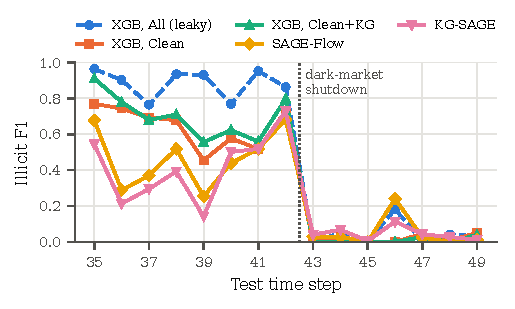
\includegraphics[width=\columnwidth]{figures/fig_per_step.pdf}
\caption{Illicit F1 per test time step (mean over seeds). All models collapse
after the dark-market shutdown at step 43.}
\label{fig:perstep}
\end{figure}

\subsection{Class imbalance (RQ2)}
\begin{table}[t]
\caption{Imbalance strategies on Clean+KG features (test F1; three seeds). PR-AUC does not depend on the threshold.}
\label{tab:imbalance}
\centering
\footnotesize
\setlength{\tabcolsep}{3pt}
\begin{tabular}{@{}llccc@{}}
\toprule
Model & Strategy & F1 @0.5 & F1 @val & PR-AUC \\
\midrule
XGB & None & 0.214\,$\pm$\,0.371 & 0.563\,$\pm$\,0.076 & 0.583\,$\pm$\,0.076 \\
XGB & Class weights & 0.609\,$\pm$\,0.010 & 0.652\,$\pm$\,0.003 & 0.684\,$\pm$\,0.005 \\
XGB & SMOTE & 0.623\,$\pm$\,0.012 & 0.640\,$\pm$\,0.009 & 0.683\,$\pm$\,0.004 \\
XGB & SMOTE-ENN & 0.573\,$\pm$\,0.008 & 0.658\,$\pm$\,0.006 & 0.701\,$\pm$\,0.006 \\
\midrule
RF & None & 0.594\,$\pm$\,0.003 & 0.499\,$\pm$\,0.071 & 0.598\,$\pm$\,0.002 \\
RF & Class weights & 0.616\,$\pm$\,0.003 & 0.603\,$\pm$\,0.010 & 0.624\,$\pm$\,0.003 \\
RF & SMOTE & 0.622\,$\pm$\,0.003 & 0.608\,$\pm$\,0.012 & 0.642\,$\pm$\,0.004 \\
RF & SMOTE-ENN & 0.595\,$\pm$\,0.005 & 0.616\,$\pm$\,0.004 & 0.650\,$\pm$\,0.003 \\
\bottomrule
\end{tabular}
\end{table}
Table~\ref{tab:imbalance} shows that some correction for imbalance is
essential: an uncorrected XGBoost model at the default threshold collapses on
some seeds (F1 $0.21\pm0.37$). With correction, the strategies are close.
For XGBoost, class weighting and SMOTE-ENN with a validation-tuned threshold
are statistically tied (F1 0.652 and 0.658), and SMOTE-ENN gives the highest
PR-AUC (0.701). For RF, all corrections reach F1 0.60--0.62. Tuning the
threshold on the validation window matters more than the choice of
resampling method for XGBoost, while for RF the default threshold is already
adequate once classes are re-weighted. Oversampling cannot be applied to the
graph models, so class weighting with threshold tuning is the strategy that
transfers across both families.

\subsection{Explanations (RQ3)}
\begin{figure}[t]
\centering
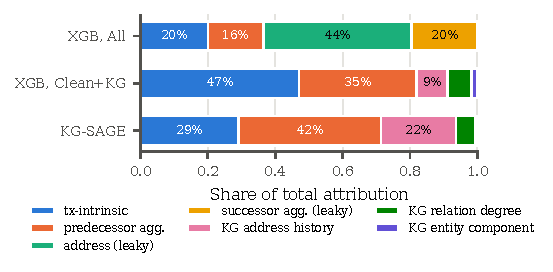
\includegraphics[width=\columnwidth]{figures/fig_attribution.pdf}
\caption{Share of total attribution per feature group: TreeSHAP for XGBoost,
gradient$\times$input for KG-SAGE (test period, seed 0).}
\label{fig:attr}
\end{figure}
Fig.~\ref{fig:attr} makes the leakage visible: XGBoost trained on
\textsc{All} features places \ShapAllLeaky{} of its attribution on the leaky
groups, \ShapAllAddr{} on address statistics computed after the test period
alone. With \textsc{Clean+KG} inputs, the KG features receive \ShapCleanKgKg{}
of the XGBoost attribution, led by the \texttt{CO\_RECEIVE} degree and the age
of the input addresses, while the transaction's own size, fee and value
statistics remain the strongest signals. KG-SAGE relies more on the graph
(\GxiKg{} of its attribution), above all on address history
(\GxiAddrHist{}, against \ShapCleanKgAddrHist{} for XGBoost). The two families
agree only moderately (Spearman $\rho=\ExplainRho$ over all features,
\ExplainOverlap{} of the top-10 features shared). Because address age and
reuse change systematically over time, the stronger reliance of the graph
model on address history is consistent with its weaker transfer to the test
period. Feature names remain those of the dataset; the semantics recovered
in~\cite{safar2026} make them interpretable (\eg\ Local~1--21 are value, fee
and input/output statistics).

\subsection{Computational cost (RQ4)}
All experiments ran on a laptop CPU. Tree ensembles on \textsc{Clean+KG}
features train in about \XgbCleanKgFit{}\,s (XGBoost) and \RfCleanKgFit{}\,s
(RF); building the TS-KG and its 15 features takes under five seconds. The graph
models are one to two orders of magnitude more expensive: \MlpFit{}\,s for the
MLP, \SageFlowFit{}\,s for SAGE-Flow and \KgSageFit{}\,s for KG-SAGE per run,
after pruning single-transaction address instances and replacing generic
scatter operations with sparse matrix products, without which a KG-SAGE epoch
took about 18\,s. Under a CPU budget, one of the cheapest models is also the most
accurate leakage-controlled one.
